\documentclass[11pt,a4paper]{article}

\usepackage[T1]{fontenc}
\usepackage[utf8]{inputenc}
\usepackage{lmodern}
\usepackage{amsmath,amssymb,mathtools}
\usepackage{booktabs}
\usepackage{tabularx}
\usepackage{graphicx}
\usepackage{xcolor}
\usepackage{geometry}
\usepackage{microtype}
\usepackage{fancyhdr}
\usepackage{lastpage}
\usepackage{placeins}
\usepackage{float}
\usepackage[hidelinks]{hyperref}

\geometry{margin=24mm,headheight=14pt}
\setlength{\parindent}{0pt}
\setlength{\parskip}{0.45em}
\graphicspath{{figures/}}

\definecolor{kthblue}{HTML}{004791}
\hypersetup{
  colorlinks=true,
  linkcolor=kthblue,
  urlcolor=kthblue,
  pdftitle={SF2527 Computer Exercise 1},
  pdfauthor={Student group}
}

\pagestyle{fancy}
\fancyhf{}
\lhead{SF2527 -- Computer Exercise 1}
\rhead{HT26}
\cfoot{\thepage\ of \pageref*{LastPage}}

\newcommand{\R}{\mathbb{R}}
\newcommand{\norm}[1]{\left\lVert #1\right\rVert_2}
\newcommand{\matlab}{\textsc{Matlab}}
\newcommand{\dd}{\,\mathrm{d}}
\numberwithin{equation}{section}
\renewcommand{\arraystretch}{1.15}


\newcommand{\coursename}{SF2527 Numerical Methods for Differential Equations I}
\newcommand{\exercisetitle}{Computer Exercise 1}
\newcommand{\exercisesubtitle}{Ordinary Differential Equations and Elliptic Equations}

\IfFileExists{student_info.tex}{
  \input{student_info}
}{
  \newcommand{\groupname}{SF2527 CE1 1}
\newcommand{\studentone}{Lukas Sönnergren}
\newcommand{\studentoneid}{\rule{24mm}{0.4pt}}
\newcommand{\studentoneemail}{\rule{35mm}{0.4pt}}
\newcommand{\studenttwo}{Tage Sköldefors}
\newcommand{\studenttwoid}{\rule{24mm}{0.4pt}}
\newcommand{\studenttwoemail}{\rule{35mm}{0.4pt}}

}

\begin{document}

\hypersetup{pageanchor=false}
\begin{titlepage}
  \centering
  {\Large KTH Royal Institute of Technology\par}
  \vspace{1.2cm}
  {\large \coursename\par}
  \vspace{2.2cm}
  {\Huge\bfseries \exercisetitle\par}
  \vspace{0.5cm}
  {\LARGE \exercisesubtitle\par}
  \vfill

  \begin{tabular}{@{}ll@{}}
    \textbf{Exercise number:} & Computer Exercise 1 \\
    \textbf{Group:} & \groupname
  \end{tabular}

  \vspace{1.2cm}
  \begin{tabularx}{0.96\textwidth}{@{}>{\bfseries}lXXX@{}}
    \toprule
    Student & Name & Personal number & Email \\
    \midrule
    1 & \studentone & \studentoneid & \studentoneemail \\
    2 & \studenttwo & \studenttwoid & \studenttwoemail \\
    \bottomrule
  \end{tabularx}

  \vfill
  {\large HT26\par}
  \vspace{0.25cm}
  {\large \today\par}
\end{titlepage}

\hypersetup{pageanchor=true}
\pagenumbering{roman}
\tableofcontents
\clearpage

\pagenumbering{arabic}
\section{Runge--Kutta accuracy and stability}

The method used throughout Parts 1 and 2 is
\begin{align}
 k_1&=f(t_n,u_n), &
 k_2&=f(t_n+h,u_n+hk_1),\\
 k_3&=f\!\left(t_n+\frac h2,u_n+\frac h4k_1+\frac h4k_2\right), &
 u_{n+1}&=u_n+\frac h6(k_1+k_2+4k_3).
\end{align}
It is an explicit three-stage, one-step Runge--Kutta method.

\subsection{Landau--Lifshitz system}

Let
\[
 a=\frac14\begin{bmatrix}1\\ \sqrt{11}\\2\end{bmatrix},\qquad
 C=\frac14\begin{bmatrix}
 0&-2&\sqrt{11}\\
 2&0&-1\\
 -\sqrt{11}&1&0
 \end{bmatrix}.
\]
Since $Cm=a\times m$, the ODE is
\[
 m'=Am,\qquad A=C+\alpha C^2,\qquad
 \alpha=0.07,\qquad m(0)=\begin{bmatrix}0&0&1\end{bmatrix}^{\mathsf T}.
\]

\begin{figure}[htbp]
\centering
\begin{minipage}{0.49\linewidth}
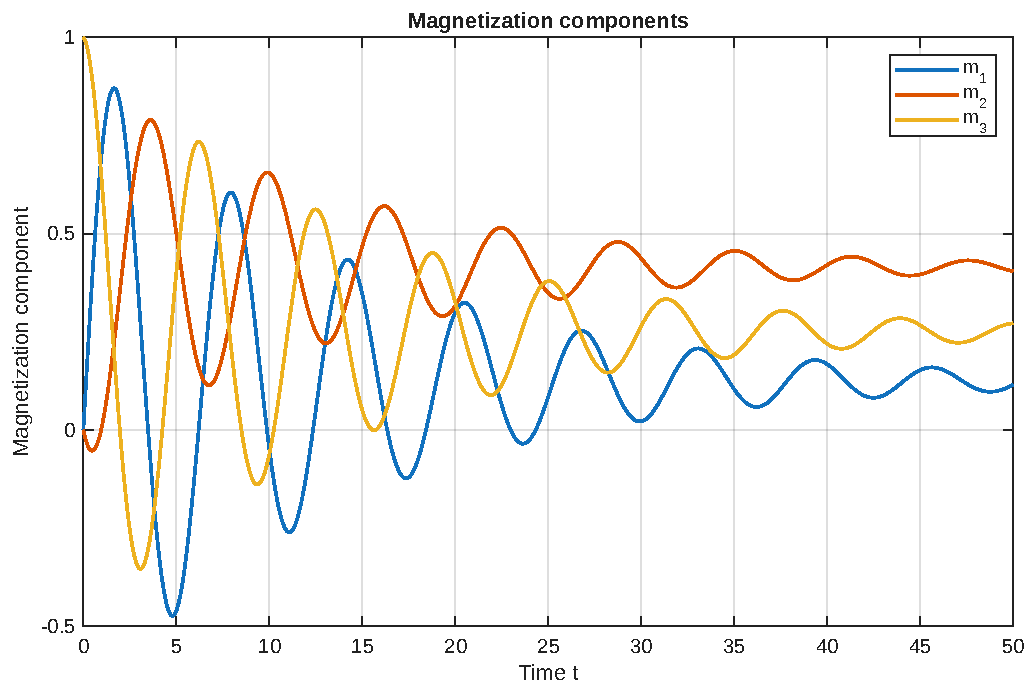
\includegraphics[width=\linewidth]{part1_components.pdf}
\end{minipage}
\begin{minipage}{0.49\linewidth}
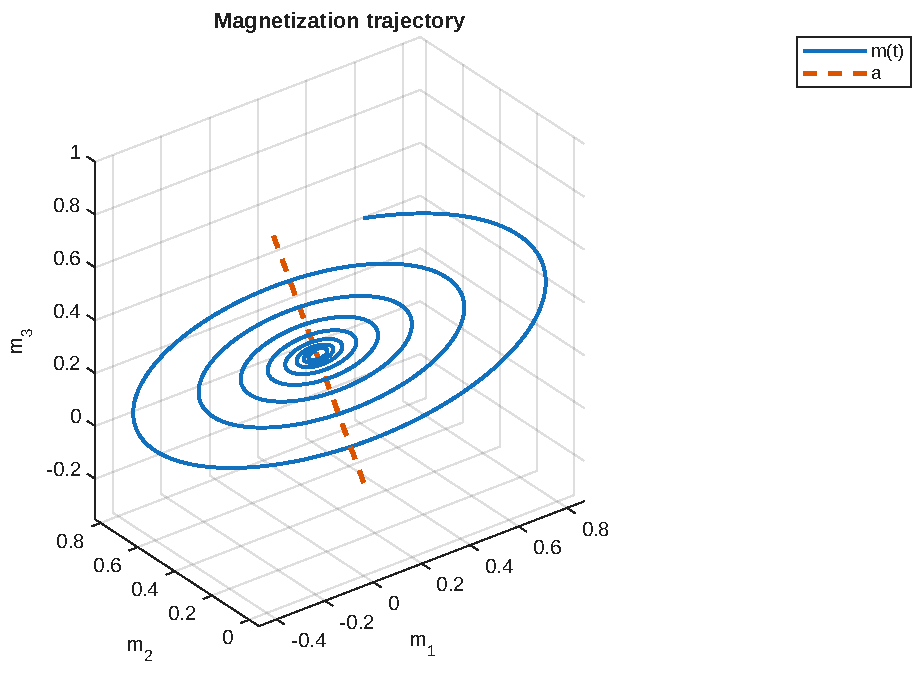
\includegraphics[width=\linewidth]{part1_trajectory.pdf}
\end{minipage}
\caption{Magnetization components and trajectory for $0\leq t\leq50$ with $h=0.01$.}
\end{figure}

The scalar product $a^{\mathsf T}m(t)=a^{\mathsf T}m(0)=1/2$ is constant. Thus the
trajectory lies in an affine plane normal to $a$. The perpendicular component
is damped and
\[
 m(t)\longrightarrow (a^{\mathsf T}m(0))a=\frac12a,
\]
which agrees with the plots.

\subsection{Order of accuracy}

For $N=50,100,200,400,800,1600$, let $h=50/N$ and
\[
 d_N=\norm{\widetilde m_N(50)-\widetilde m_{2N}(50)}.
\]
The fitted log--log slope is
\[
 \boxed{p=2.994893},
\]
confirming third-order global accuracy.

\begin{figure}[htbp]
\centering
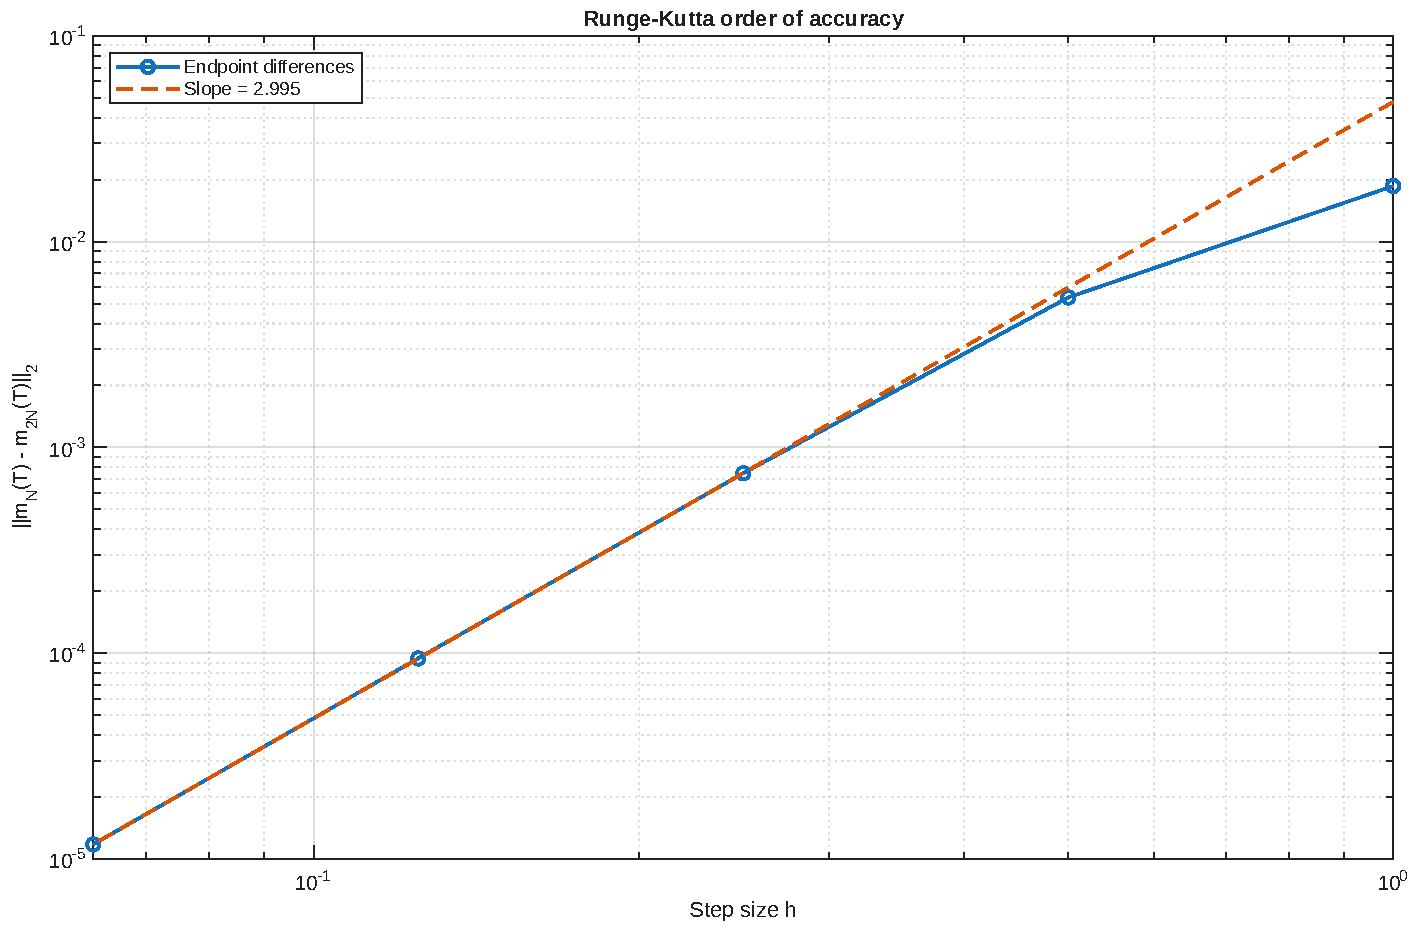
\includegraphics[width=0.72\linewidth]{part1_order.pdf}
\caption{Endpoint differences and fitted order.}
\end{figure}

\subsection{Stability limit}

The eigenvalues of $A$ are
\[
 \lambda_1=0,\qquad \lambda_{2,3}=-0.07\pm i.
\]
The stability function is
\[
 R(z)=1+z+\frac{z^2}{2}+\frac{z^3}{6}.
\]
Stability requires $|R(h\lambda_j)|\leq1$ for every eigenvalue. The zero
eigenvalue gives $R(0)=1$. For $\lambda=-0.07+i$, the first positive root of
\[
 |R(h\lambda)|-1=0
\]
was computed with \texttt{fzero} on $[2,2.5]$, giving
\[
 \boxed{h_0=2.055596}.
\]
The run with $h=2$ is stable, while $h=50/24=2.083333$ is unstable.

\begin{figure}[htbp]
\centering
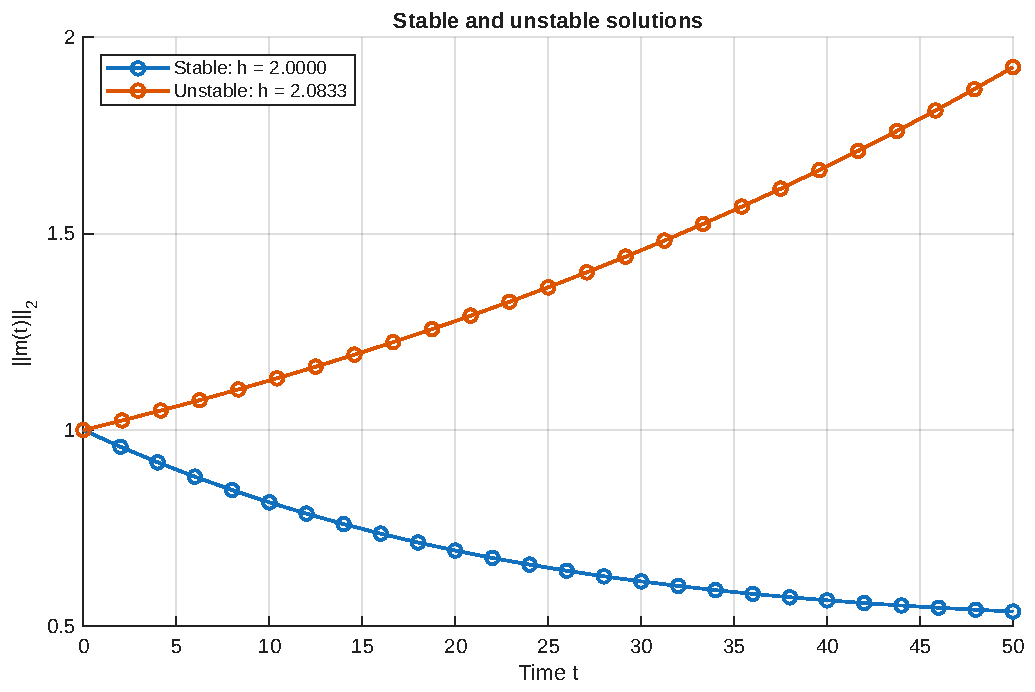
\includegraphics[width=0.72\linewidth]{part1_stable_unstable.pdf}
\caption{Stable and unstable solutions on opposite sides of $h_0$.}
\end{figure}

\FloatBarrier
\section{Robertson's stiff system}

The concentrations $x=[x_A,x_B,x_C]^{\mathsf T}$ satisfy
\begin{align}
 x_A'&=-r_1x_A+r_2x_Bx_C,\\
 x_B'&=r_1x_A-r_2x_Bx_C-r_3x_B^2,\\
 x_C'&=r_3x_B^2,
\end{align}
where
\[
 r_1=5.0\times10^{-2},\qquad r_2=1.2\times10^4,
 \qquad r_3=4.0\times10^7,qquad x(0)=\begin{bmatrix}1&0&0\end{bmatrix}^{\mathsf T}.
\]
The invariant $x_A+x_B+x_C=1$ was preserved numerically.

\subsection{Explicit Runge--Kutta method}

On $0\leq t\leq10$, $h=7.0\times10^{-4}$ gave a stable solution. The linear
plot hides the small intermediate concentration $x_B$; the logarithmic plot
shows its fast initial transient.

\begin{figure}[htbp]
\centering
\begin{minipage}{0.49\linewidth}
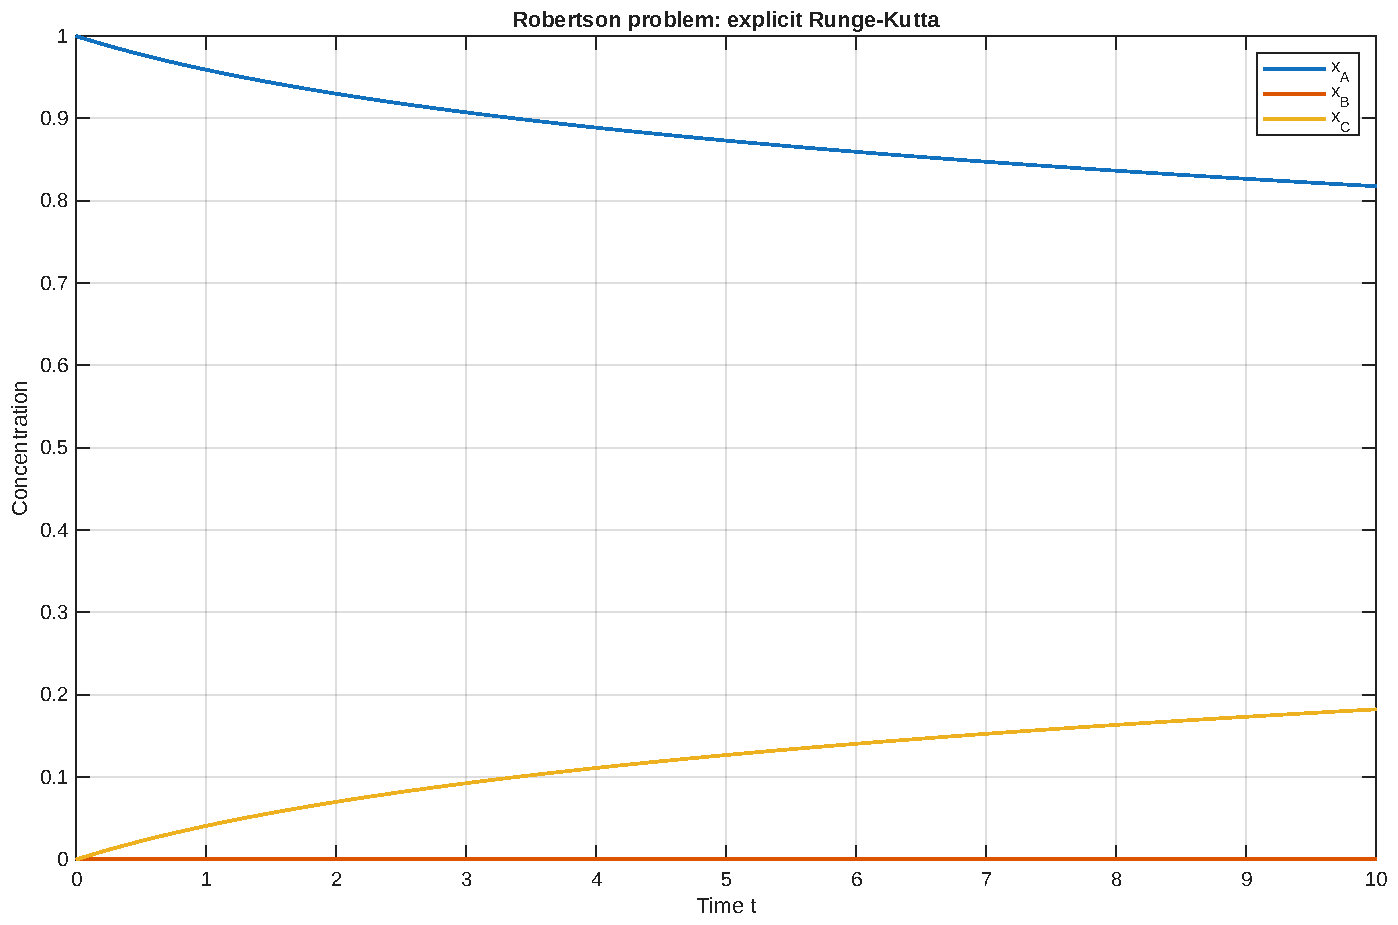
\includegraphics[width=\linewidth]{part2_rk_linear.pdf}
\end{minipage}
\begin{minipage}{0.49\linewidth}
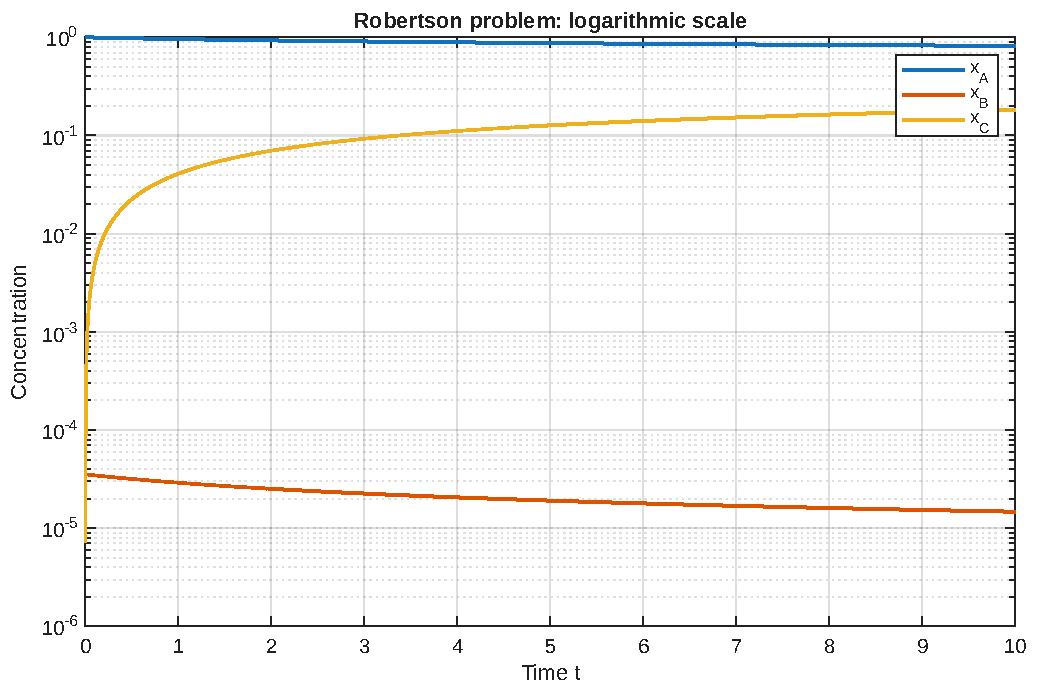
\includegraphics[width=\linewidth]{part2_rk_semilogy.pdf}
\end{minipage}
\caption{Explicit RK solution on $0\leq t\leq10$ with $h\approx7.0\times10^{-4}$.}
\end{figure}

The Jacobian is
\[
J(x)=\begin{bmatrix}
-r_1&r_2x_C&r_2x_B\\
r_1&-r_2x_C-2r_3x_B&-r_2x_B\\
0&2r_3x_B&0
\end{bmatrix}.
\]
For a perturbation $e$, $e'\approx J(x(t))e$, so local stability requires
$|R(h\lambda_j(t))|\leq1$. One eigenvalue is zero. Along the computed solution,
\[
 \max_t|\lambda_j(t)|=3365.924700.
\]
The negative real-axis boundary of the RK region gives
\[
 h_{\max}\approx7.4652\times10^{-4},
\]
in agreement with the empirical value. The restriction becomes more severe as
the large eigenvalue grows in magnitude.

\begin{figure}[htbp]
\centering
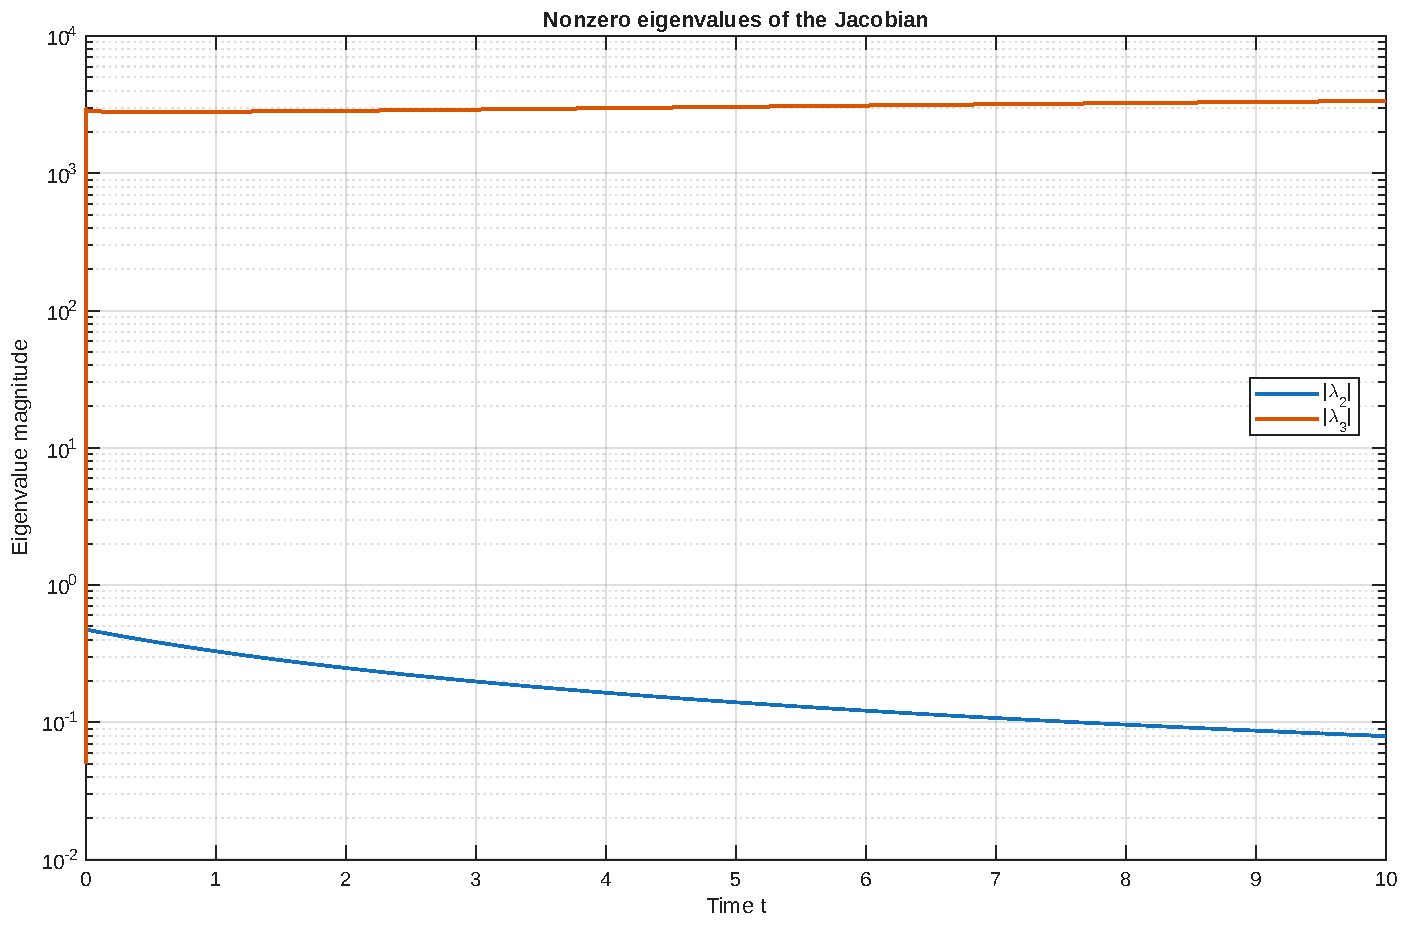
\includegraphics[width=0.72\linewidth]{part2_jacobian_eigenvalues.pdf}
\caption{Magnitudes of the two nonzero Jacobian eigenvalues.}
\end{figure}

For the long integration, only the current state was stored.
\begin{table}[htbp]
\centering
\caption{Explicit RK result at $t=1000$.}
\begin{tabular}{@{}lc@{}}
\toprule
Quantity & Value\\
\midrule
$h$ & $2.8\times10^{-4}$\\
$x_A(1000)$ & $0.293414227164$\\
$x_B(1000)$ & $1.716342048384\times10^{-6}$\\
$x_C(1000)$ & $0.706584056494$\\
Time & $2.93\ \mathrm{s}$\\
\bottomrule
\end{tabular}
\end{table}

\subsection{Implicit Euler}

Implicit Euler satisfies
\[
 u_{n+1}=u_n+hf(u_{n+1}).
\]
At each step, the supplied code solves
\[
 F(v)=v-hf(v)-u_n=0
\]
with Newton's method:
\[
 (I-hJ_f(v))d=-F(v),\qquad v\leftarrow v+d.
\]
Runs with $h=10$, $1$ and $0.1$ remained bounded. The large steps are stable but
inaccurate. The choice $h=0.1$ visually agrees with RK on $[0,10]$ and was reused
on $[0,1000]$.

\begin{figure}[htbp]
\centering
\begin{minipage}{0.49\linewidth}
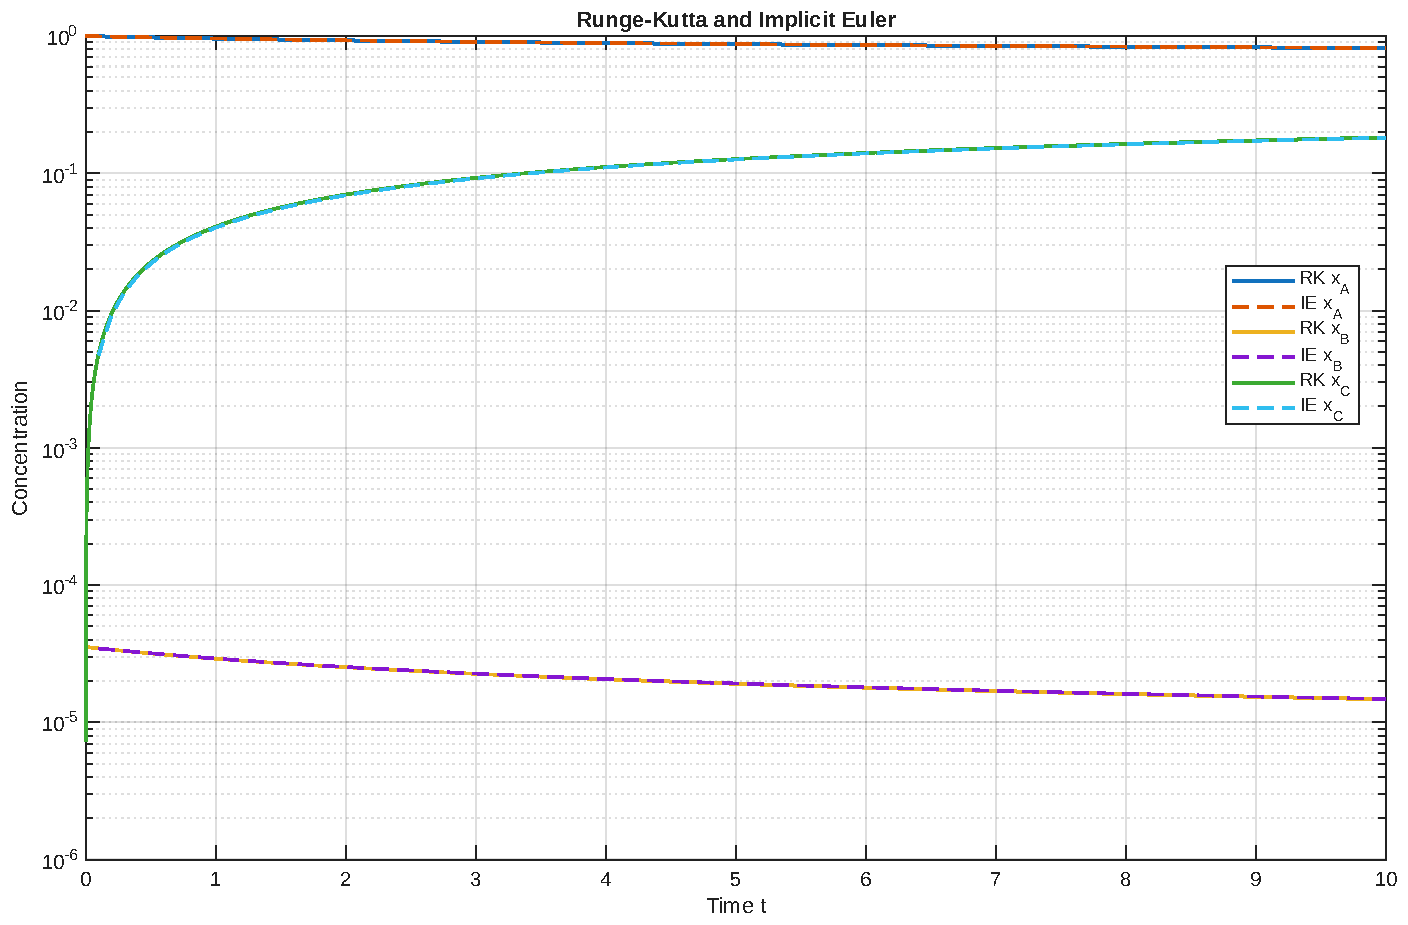
\includegraphics[width=\linewidth]{part2_rk_ie_comparison.pdf}
\end{minipage}
\begin{minipage}{0.49\linewidth}
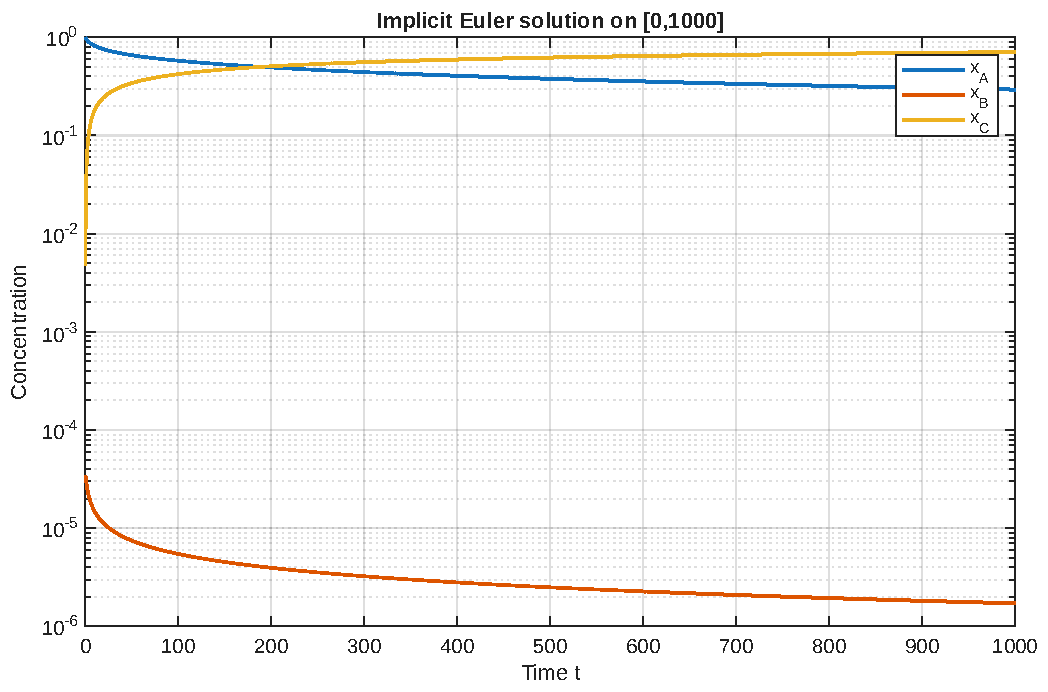
\includegraphics[width=\linewidth]{part2_implicit_euler.pdf}
\end{minipage}
\caption{Short-time RK/IE comparison and the IE solution on $[0,1000]$.}
\end{figure}

\subsection{Efficiency}

Errors were measured against the supplied reference value at $t=1000$. The IE
timing version stores only the current state.

\begin{table}[htbp]
\centering
\caption{Endpoint error and single-run computational time.}
\begin{tabular}{@{}lccc@{}}
\toprule
Method & $h$ & Error & Time (s)\\
\midrule
RK & $2.8\times10^{-4}$ & $3.06\times10^{-13}$ & $2.93$\\
IE & $1$ & $4.93\times10^{-4}$ & $0.014$\\
IE & $0.1$ & $5.03\times10^{-5}$ & $0.048$\\
IE & $0.01$ & $5.04\times10^{-6}$ & $0.409$\\
IE & $0.001$ & $5.04\times10^{-7}$ & $4.04$\\
\bottomrule
\end{tabular}
\end{table}

IE is faster for moderate accuracy because stability permits large steps. For
high accuracy, its first-order error and Newton solves dominate; RK is faster
below an error of roughly $10^{-6}$. For the nonstiff problem in Part 1, IE has
no useful stability advantage, so the higher-order explicit method is preferable.

\FloatBarrier
\section{One-dimensional convection--diffusion equation}

The problem is
\[
 -T''(z)+vT'(z)=Q(z),\qquad 0<z<1,
\]
with $T(0)=T_0$ and
\[
 -T'(1)=\alpha(v)(T(1)-T_{\mathrm{out}}),\qquad
 \alpha(v)=\sqrt{\frac{v^2}{4}+\alpha_0^2}-\frac v2.
\]
The parameters are
\[
 a=0.1,\ b=0.4,\ Q_0=7000,\ \alpha_0=50,\
 T_{\mathrm{out}}=25,\ T_0=100,
\]
and
\[
Q(z)=\begin{cases}
Q_0\sin\!\left(\dfrac{(z-a)\pi}{b-a}\right),&a\leq z\leq b,\\
0,&\text{otherwise}.
\end{cases}
\]

Let $z_j=jh$, $h=1/N$, and $U=[T_1,\ldots,T_N]^{\mathsf T}$. At
$j=1,\ldots,N-1$,
\[
 \ell T_{j-1}+dT_j+rT_{j+1}=Q(z_j),
\]
where
\[
 \ell=-\frac1{h^2}-\frac{v}{2h},\qquad
 d=\frac2{h^2},\qquad
 r=-\frac1{h^2}+\frac{v}{2h}.
\]
The known value $T_0$ is moved to the first right-hand-side entry. The
second-order outlet row is
\[
 T_{N-2}-4T_{N-1}+(3+2h\alpha)T_N=2h\alpha T_{\mathrm{out}}.
\]
The resulting sparse linear system is solved with backslash.

\subsection{Grid refinement}

\begin{figure}[htbp]
\centering
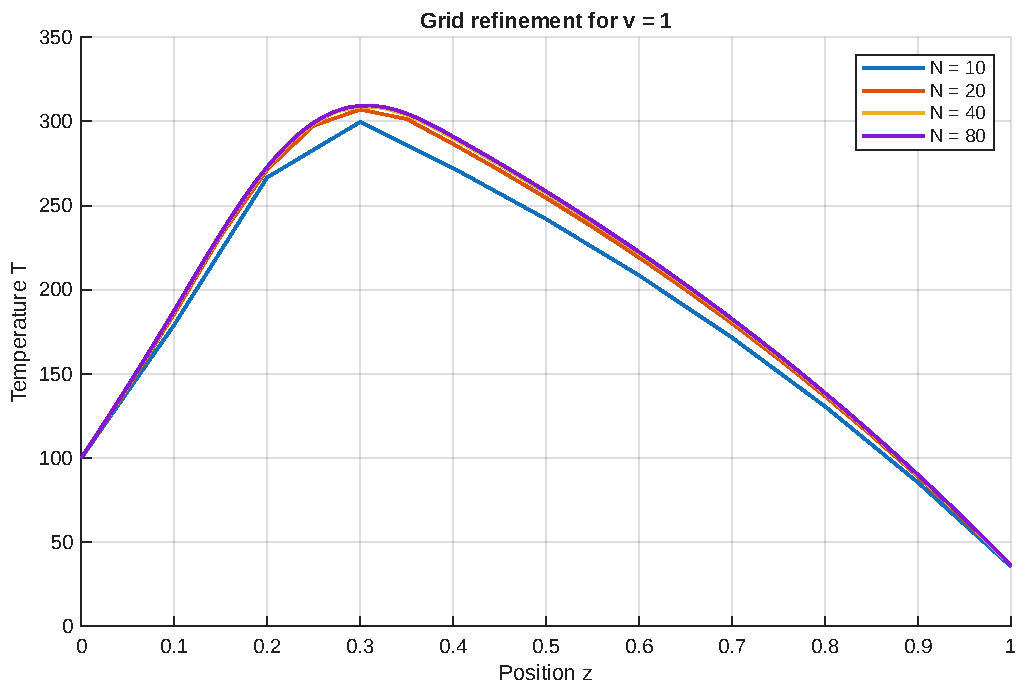
\includegraphics[width=0.74\linewidth]{part3_refinement.pdf}
\caption{Solutions for $v=1$ and $N=10,20,40,80$.}
\end{figure}

\begin{table}[htbp]
\centering
\caption{Temperature at the exact grid point $z=0.5$.}
\begin{tabular}{@{}ccc@{}}
\toprule
$N$ & $h$ & $T_h(0.5)$\\
\midrule
80 & $0.0125$ & $258.430491144194$\\
160 & $0.00625$ & $258.621578905525$\\
320 & $0.003125$ & $258.669336283685$\\
\bottomrule
\end{tabular}
\end{table}

Using successive differences gives
\[
 p=\log_2\!\left(
 \frac{|T_{80}(0.5)-T_{160}(0.5)|}
 {|T_{160}(0.5)-T_{320}(0.5)|}\right)
 =\boxed{2.000440}.
\]
The source is evaluated at the same points $z_j$ on every grid, and $z=0.5$
is read at index $j=N/2$.

\subsection{Velocity dependence}

\begin{table}[htbp]
\centering
\caption{Grids used for the velocity comparison.}
\begin{tabular}{@{}ccc@{}}
\toprule
$v$ & $N$ & $h$\\
\midrule
1 & 80 & $0.0125$\\
5 & 100 & $0.0100$\\
15 & 300 & $0.003333$\\
100 & 2000 & $0.0005$\\
\bottomrule
\end{tabular}
\end{table}

\begin{figure}[htbp]
\centering
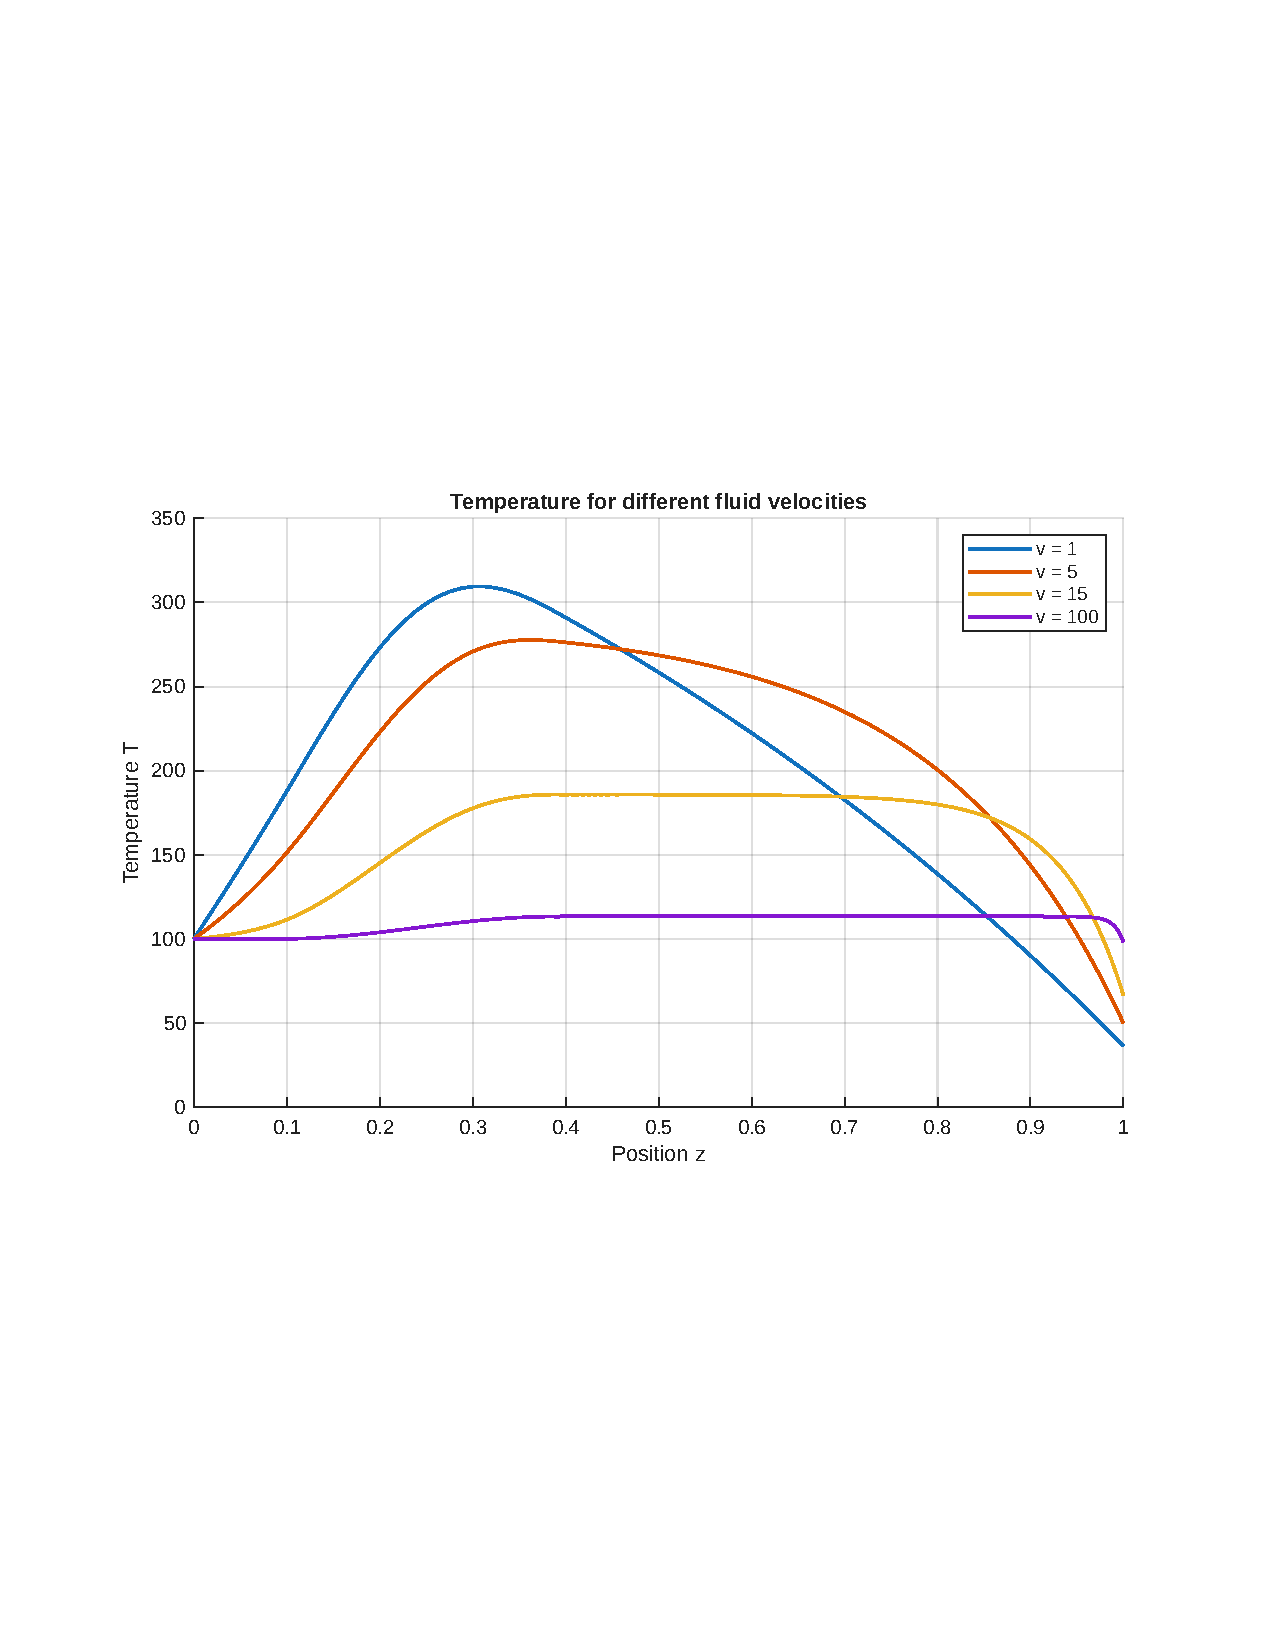
\includegraphics[width=0.74\linewidth]{part3_velocity_comparison.pdf}
\caption{Temperature profiles for $v=1,5,15,100$.}
\end{figure}

Larger $v$ transports heat downstream more rapidly, so the temperature rise is
smaller and the profile is flatter. It also produces a thinner outlet feature;
the finer grids resolve this feature without oscillations.

\FloatBarrier
\section{Two-dimensional elliptic heat equation}

The problem is
\[
 -\Delta T=f\quad\text{in }(0,12)\times(0,5),
\]
with $T(x,0)=T_{\mathrm{ext}}=25$ and homogeneous Neumann conditions on the
left, right and top boundaries. The mesh has
\[
 h=\frac{12}{N}=\frac5M.
\]

The bottom values are known. All points with $i=0,\ldots,N$ and
$j=1,\ldots,M$ are numbered by
\[
 k=i+1+(j-1)(N+1).
\]
Thus the sparse matrix has size $(N+1)M\times(N+1)M$. At an interior point,
\[
 4T_{i,j}-T_{i-1,j}-T_{i+1,j}-T_{i,j-1}-T_{i,j+1}
 =h^2f(x_i,y_j).
\]
For $j=1$, the known lower value adds $T_{\mathrm{ext}}$ to the right-hand side.
The second-order boundary rows are
\begin{align*}
 -3T_{0,j}+4T_{1,j}-T_{2,j}&=0,\\
 3T_{N,j}-4T_{N-1,j}+T_{N-2,j}&=0,\\
 3T_{i,M}-4T_{i,M-1}+T_{i,M-2}&=0.
\end{align*}
The upper corners use the side rows. This gives one equation for every unknown.

\subsection{Constant source}

For $f\equiv2$ and $h=0.2$, the computed value is
\[
 \boxed{T_h(6,2)=41.000000000000}.
\]

\begin{figure}[htbp]
\centering
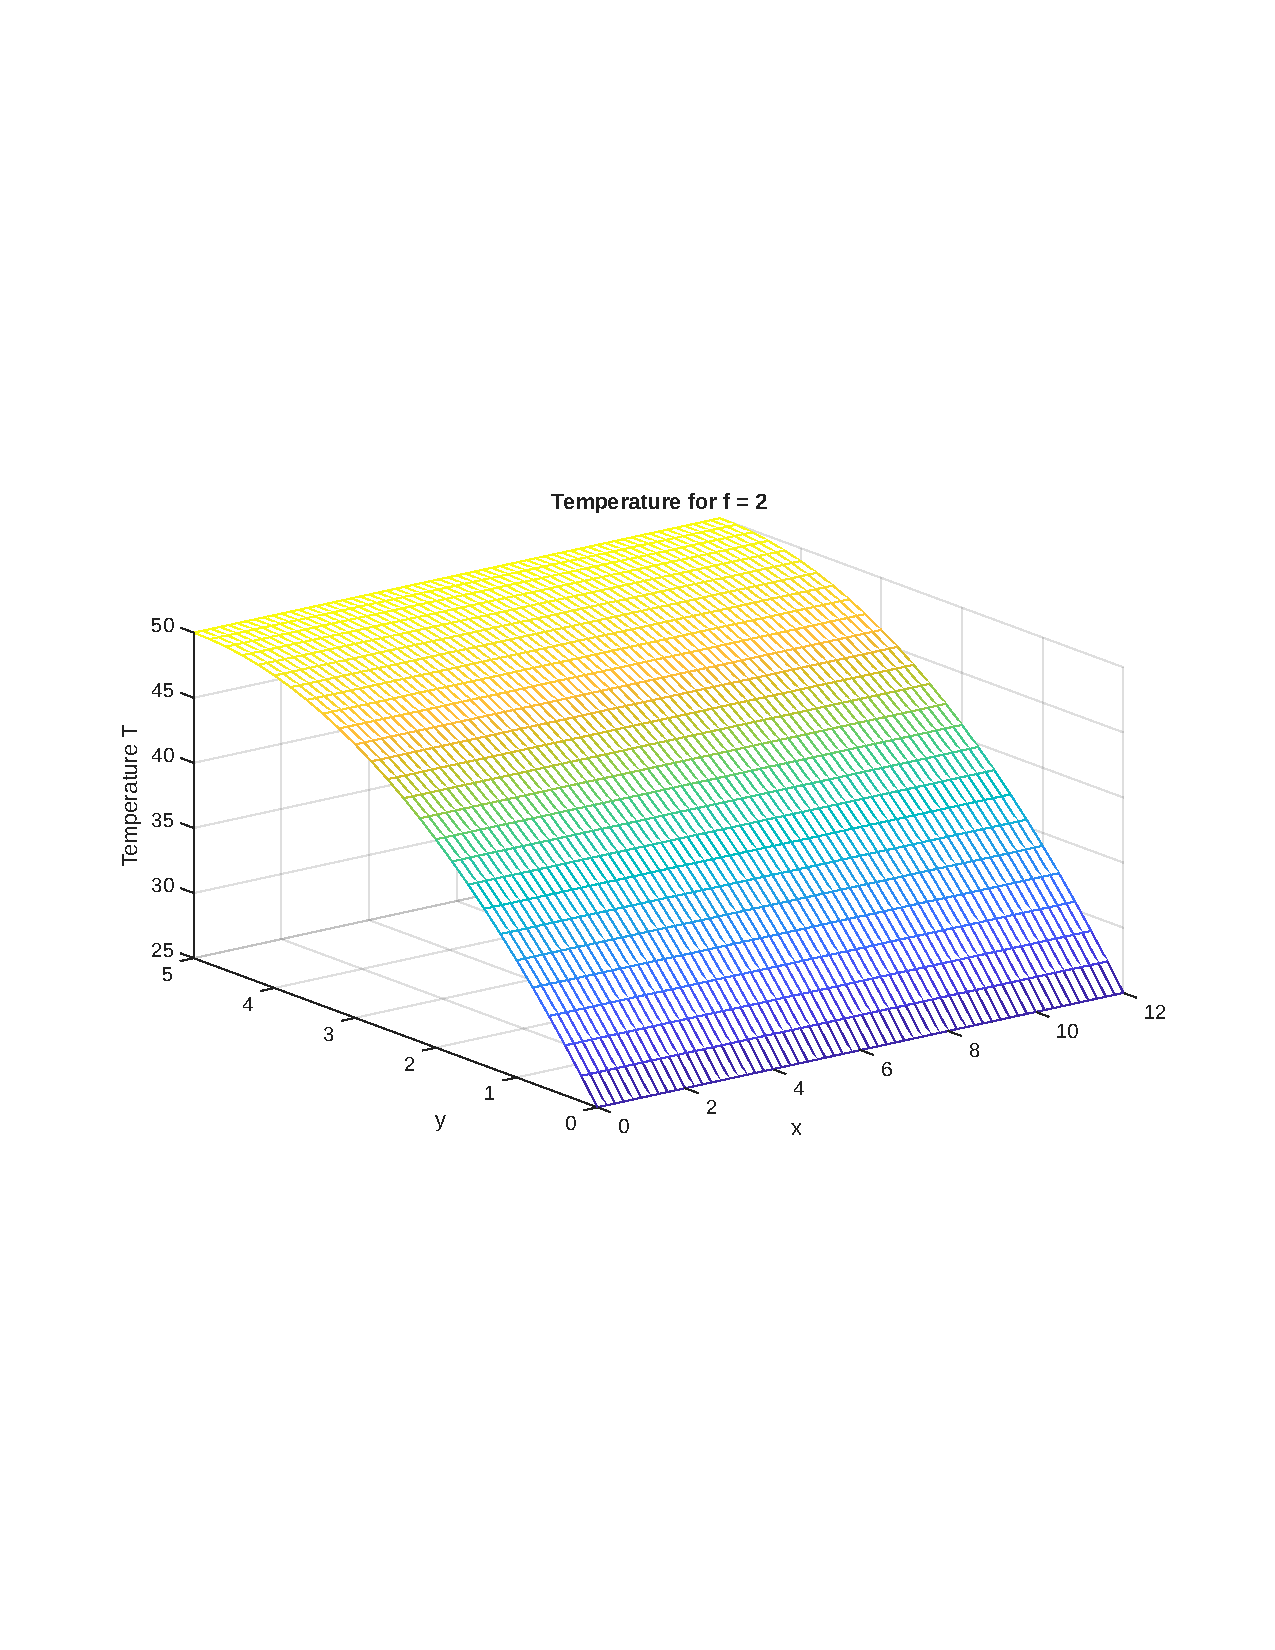
\includegraphics[width=0.72\linewidth]{part4_constant_mesh.pdf}
\caption{Numerical solution for $f\equiv2$ and $h=0.2$.}
\end{figure}

For an exact solution $T=c_0+c_1y+c_2y^2$, the PDE and boundary conditions give
\[
 -2c_2=2,\qquad c_0=25,\qquad c_1+10c_2=0.
\]
Hence
\[
 \boxed{T(x,y)=25+10y-y^2},\qquad T(6,2)=41.
\]
The central difference satisfies
\[
 \frac{g(x+h)-2g(x)+g(x-h)}{h^2}
 =g''(x)+\frac{h^2}{12}g^{(4)}(x)+O(h^4).
\]
For a quadratic, $g^{(3)}=g^{(4)}=0$. Both the interior stencil and the
one-sided boundary derivatives are therefore exact. The observed difference
at $(6,2)$ was $3.70\times10^{-13}$, due only to floating-point arithmetic.

\subsection{Localized source}

For
\[
 f(x,y)=100\exp\!\left(-\frac12(x-4)^2-4(y-1)^2\right),
\]
the same matrix construction is used with a new right-hand side.

\begin{table}[htbp]
\centering
\caption{Localized-source values at $(6,2)$.}
\begin{tabular}{@{}cccc@{}}
\toprule
$h$ & $N$ & $M$ & $T_h(6,2)$\\
\midrule
0.20 & 60 & 25 & $47.219954048124$\\
0.10 & 120 & 50 & $47.224023288355$\\
0.05 & 240 & 100 & $47.224999298104$\\
\bottomrule
\end{tabular}
\end{table}

The successive-difference estimate is
\[
 \boxed{p=2.059792},
\]
which is consistent with second-order convergence. For the finest grid the
system has $24100$ unknowns, so sparse storage is essential.

\begin{figure}[htbp]
\centering
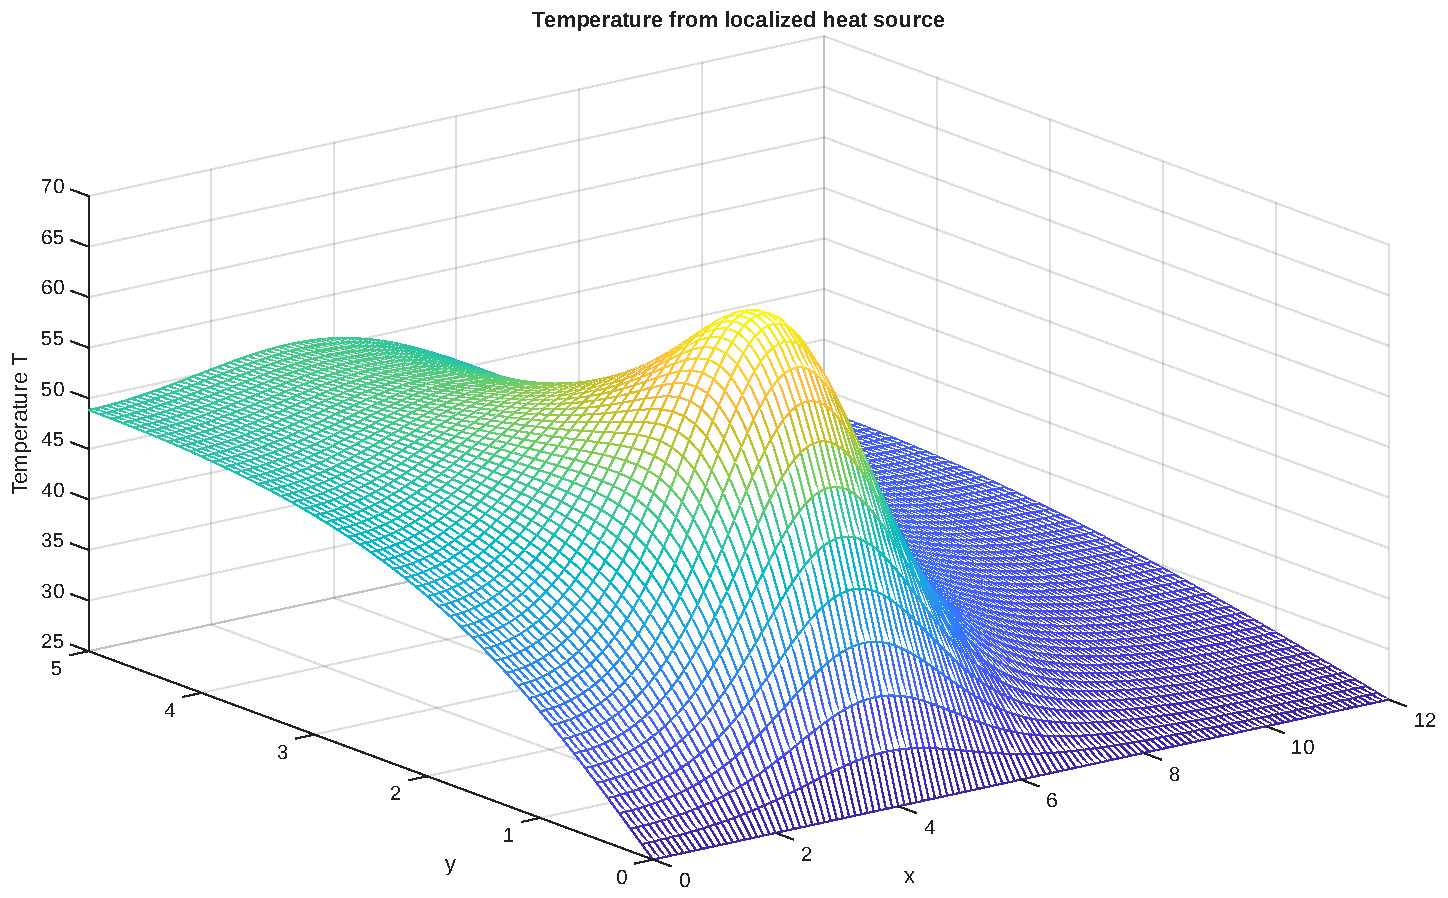
\includegraphics[width=0.72\linewidth]{part4_localized_mesh.pdf}
\caption{Mesh plot for the localized source with $h=0.1$.}
\end{figure}

\begin{figure}[htbp]
\centering
\begin{minipage}{0.49\linewidth}
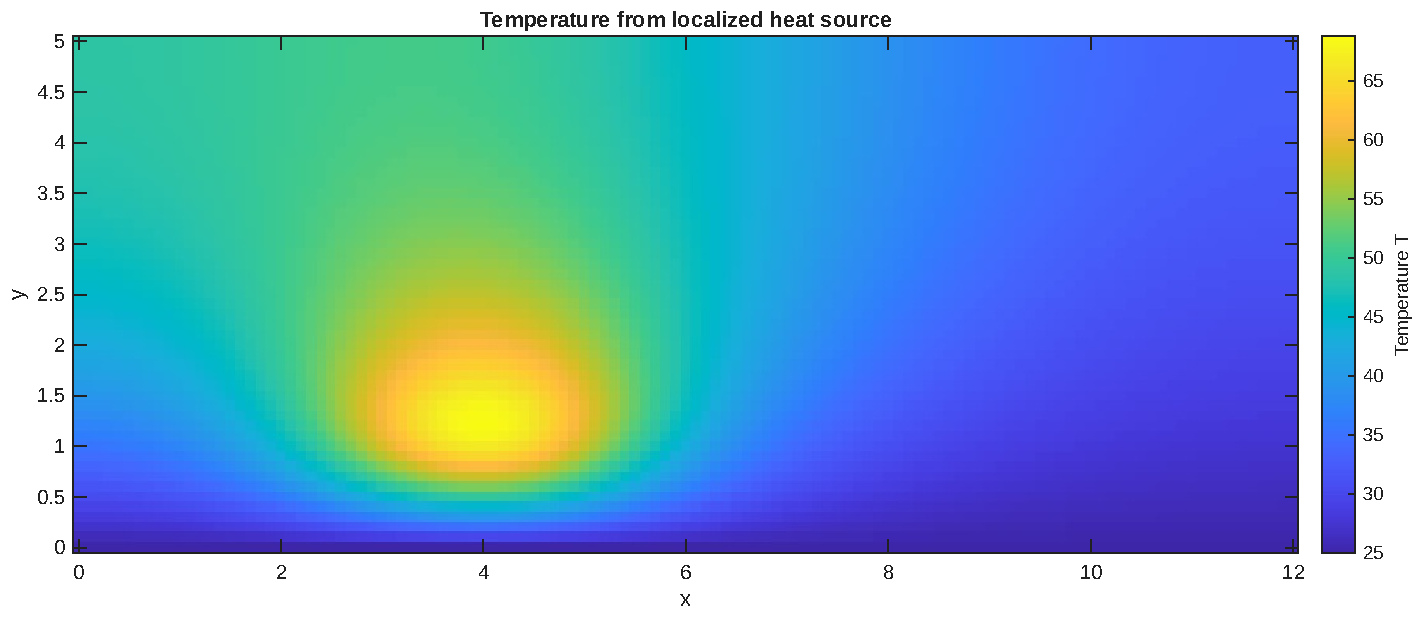
\includegraphics[width=\linewidth]{part4_localized_imagesc.pdf}
\end{minipage}
\begin{minipage}{0.49\linewidth}
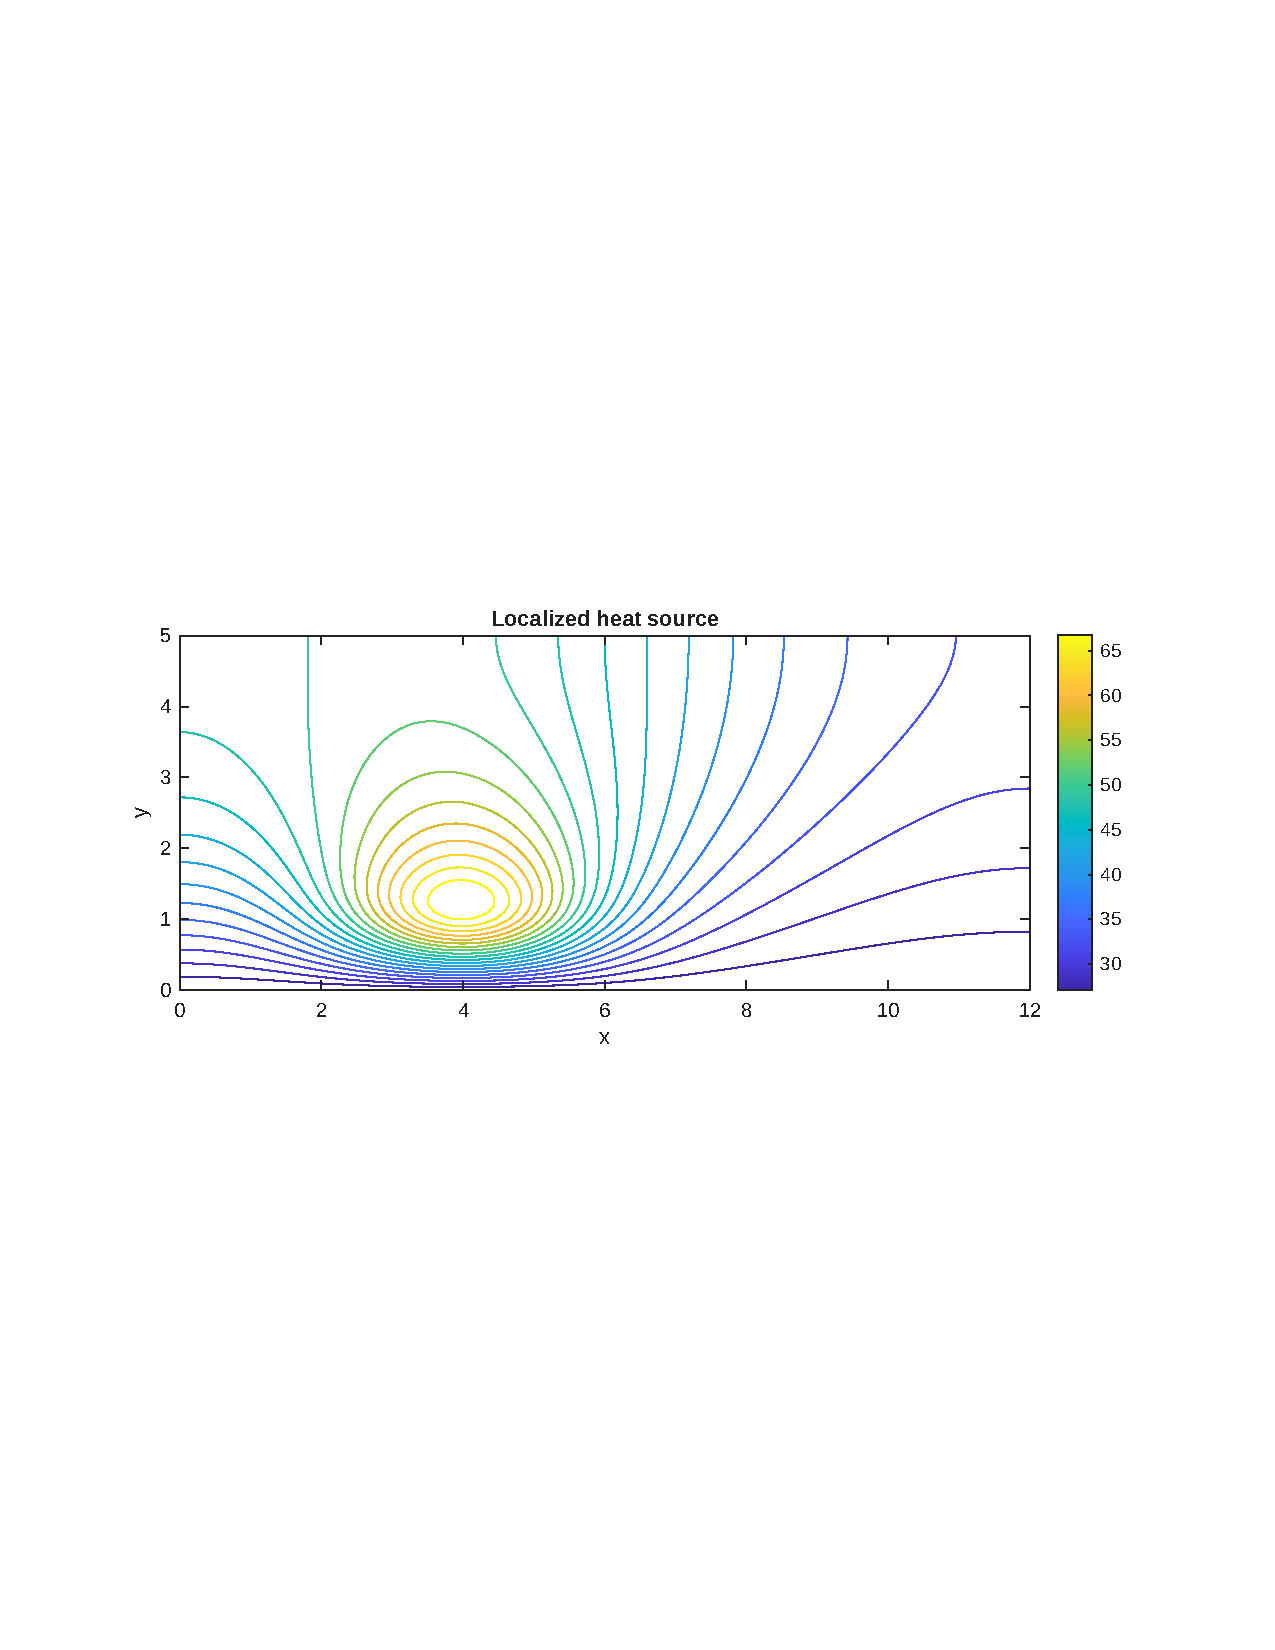
\includegraphics[width=\linewidth]{part4_localized_contour.pdf}
\end{minipage}
\caption{Image and contour views for $h=0.1$. The hot region is centred near the source at $(4,1)$.}
\end{figure}

\FloatBarrier
\section{Conclusions}

The RK method showed third-order accuracy and the predicted stability limit.
For the stiff Robertson problem, implicit Euler was efficient at moderate
accuracy, while RK was preferable for high accuracy. Both finite-difference
implementations showed second-order convergence. The analytic quadratic in
Part 4 provided an exact verification of the two-dimensional matrix assembly.

\section*{Submitted MATLAB files}

\begin{itemize}
\item \texttt{ce1\_part1\_rk\_landau\_lifshitz.m}, \texttt{rk3\_step.m}
\item \texttt{ce1\_part2\_robertson.m}, \texttt{impeuler.m}, \texttt{impeuler\_nosave.m}
\item \texttt{ce1\_part3\_convection\_diffusion\_1d.m}, \texttt{solve\_convection\_diffusion.m}
\item \texttt{ce1\_part4\_elliptic\_heat\_2d.m}, \texttt{solve\_heat\_2d.m}
\end{itemize}


\end{document}
